\section{Paleo-sea level compilations}

This is a list of paleo-sea level compilations, which served as the basis for this report. We acknowledge the hard work of the people compiling the data, as well as acknowledging those who collected the original data.

\subsection{North America}

\begin{itemize}
  \item Canada and Greenland - A.S. Dyke and T.S. James (unpublished, though some of it was summarized in \citet{DykePeltier2000})
  \item Eastern Canada - \citet{VacchiEtal2018}
  \item Hudson Bay - \citet{SimonEtal2016}
  \item Hudson Bay and northern mainland Canada - \citet{GowanEtal2016}
\end{itemize}

There were many data that refered just to compilations rather than the original sources. I have tried to track down the original sources as much as possible, but in some cases it was not possible, as they were neither listed in the Vacchi compilation nor the Dyke and James compilation.

The compilation of sea level indicators in the eastern United States was done by \citet{EngelhartHorton2012}. Thanks to Simon Engelhart for sending me a copy of the dataset with the reservoir corrections used for marine organisms.

The MIS 3-5 data from the east coast of the United States was compiled by \citet{PicoEtal2017}.

\subsection{Europe}

\label{sec:Europe}

The Baltic Sea sea level indicators are from \citep{RosentauEtal2021}. Note that some of the regions that they designated were really large with the gradient of the GIA, so I made smaller regions. This is why the regions in this report do not correspond to theirs in many places. Also note that Rosentau \emph{et al} chose to enter the radiocarbon dates for {\AA}ngermanland as pre-calibrated dates. I have not changed them.


Scandinavia sea level indicators are from and unpublished compilation by Jan Mangerud, Kristian Vasskog and \O{}ystein Lohne. Since this compilation is not available yet, the data points are not uploaded to the main Github repository. Some parts of the compilation can be found in:

\begin{itemize}
  \item Svalbard - \citet{BondevikEtal1995}
  \item Northern Europe - \citet{FormanEtal2004}
  \item Norway - \citet{LohneEtal2007,RomundsetEtal2010,RomundsetEtal2011,RomundsetEtal2015,RomundsetEtal2018,VasskogEtal2019}
\end{itemize}

The main compilation for the North Sea is by \citet{VinkEtal2007}. Though this predates the HOLSEA project, they use the indicative meaning concept and have a rigorous assessment of error, and is compatible with it. For Rotterdam, Netherlands, there is a HOLSEA compilation by \citet{HijmaCohen2019}. In Langeoog, there is a HOLSEA dataset by \citet{BungenstockEtal2021}. I have also included HOLSEA formatted data from Norderney \citep{SchederEtal2022}. Western Denmark does not a HOLSEA formatted compilation, so I added data compiled by \citet{GehrelsEtal2006} and \citet{JessenEtal2019}.


\subsection{Eurasian Arctic}

The sea level indicators for northern Norway and Svalbard are from and unpublished compilation by Jan Mangerud, Kristian Vasskog and \O{}ystein Lohne (see details in Section~\ref{sec:Europe}).

The compilation of sea level indicators for northern Russia comes from \citet{BaranskayaEtal2018}. Thank you to Alisa V. Baranskaya for sending the references (including translations from Russian) that were missing from the published compilation.

\subsection{Southeastern Asia}

The sea level indicators from southeastern Asia were compiled by \citet{MannEtal2019}.

\subsection{Tropical Corals}

Corals from tropical regions were compiled by \citet{HibbertEtal2016}. In this report, we have taken indicators for Huon Peninsula, Vanuatu and French Polynesia from this database.

\subsection{Antarctica}

Currently, I have included two compilations from Antarctica. The compilation by \citet{IshiwaEtal2021} is focused on East Antarctica and includes MIS 3 data. The other is by \citet{BriggsTarasov2013}, and includes data from both West and East Antarctica for the Holocene. I also added a couple of sites not included in these compilations, including \citet{HjortEtal1997} and \citet{BraddockEtal2022}.

\subsection{Australia}

The main compilation of Australia is from \citet{LewisEtal2013}. Thanks goes to Stephen E. Lewis, who kindly sent me the spreadsheets from this compilation and allowed me to include them in this database. This database was actually kind of a ``database of databases", which put together state databases, including New South Wales \citep{SlossEtal2007}, Queensland \citep{LarcombeEtal1995} and South Australia \citep{BelperioEtal2002}. Tasmania was not included in the Lewis paper because of a lack of studies. There is a compilation of Tasmania in \citet{Morrison2019}, which I have included. In addition, I have included the Great Barrier Reef data from \citet{YokoyamaEtal2018} and Bonaparte Gulf from \citet{YokoyamaEtal2000} and \citet{IshiwaEtal2019}.

\clearpage

\subsection{Data locations}

\begin{figure}[h]
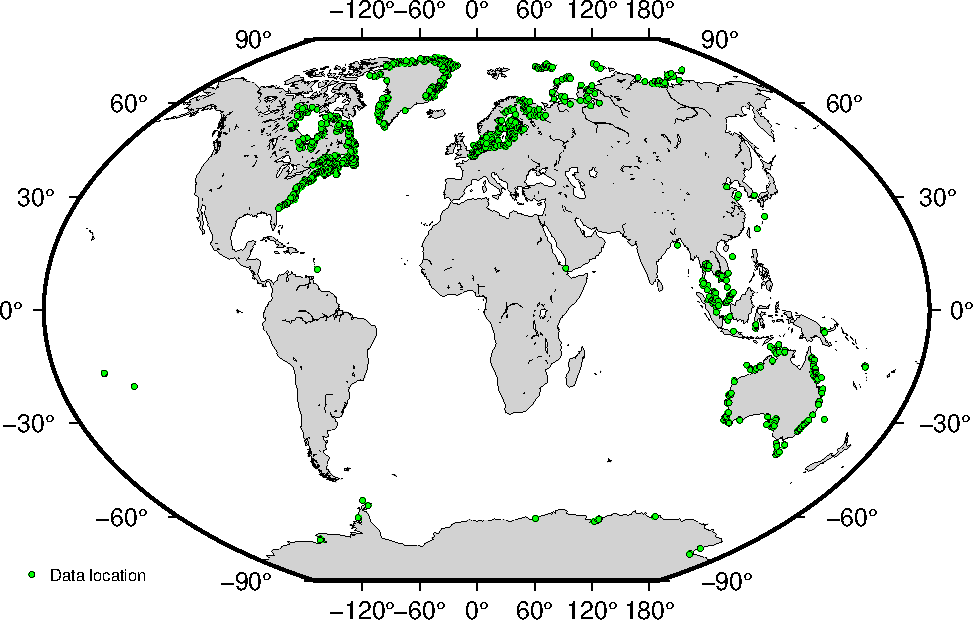
\includegraphics[width=\textwidth]{../GIS/data_map.pdf}
\caption{Map showing the location of data entered into the database.}
\label{fig:data_map}
\end{figure}

\clearpage
